\chapter{信号与系统}

\section{信号与系统}

\begin{proposition}

    考虑离散时间信号
    \[x[n] = 1 - \sum\limits_{k = 3}^{\infty}{\delta[n - 1 - k]}\]
    确定整数$M$和$n_0$的值,使得$x[n]$能表示为
    \[x[n] = u[Mn - n_0]\]

\end{proposition}


\begin{proof}

    由题设知,
    \[x[n] = 1 - \sum\limits_{k = 3}^{\infty}{\delta[n - 1 - k]} = 1 - \sum\limits_{k = 4}^{\infty}{\delta[n - k]}\]
    即
    $$x[n] = \left\{
                \begin{aligned}
                    & 1, &n \leq 3 \\
                    & 0 , &x \geq 4 \\
                \end{aligned}
                \right.
    $$
    因此
    \[x[n] = u[-n + 3]\]
    所以,$M = -1$,$n_0 = -3$.

\end{proof}

\section{线性时不变系统}

\begin{proposition}

    考虑一个离散时间系统$X_1$,其单位脉冲响应为
    \[h[n] = \left( \dfrac{1}{5} \right)^nu[n]\]

    \begin{enumerate}
        
        \item 求整数$A$以满足$h[n] - Ah[n - 1] = \delta[n]$.
        
        \item 利用\textup{(a)}的结果,求$S_1$的逆系统$S_2$是线性时不变的单位脉冲响应$g[n]$.
        
    \end{enumerate}

\end{proposition}

\begin{proof}
    
    \begin{enumerate}
        
        \item 
            由题设,因为
            \[h[n] - Ah[n - 1]  = \left( \dfrac{1}{5} \right)^nu[n] - A \left( \dfrac{1}{5} \right)^{n - 1}u[n - 1]\]
            即
            $$h[n] - Ah[n - 1] = \left\{
                        \begin{aligned}
                            & \left( dfrac{1}{5} \right)^n - A \left( \dfrac{1}{5} \right)^{n - 1}, && n \geq 0 \\
                            & 1, && n = 0 \\
                            & 0, && n \leq -1 
                        \end{aligned}
                        \right.
            $$
            所以,$A = \dfrac{1}{5}$

        \item 
            即求$g[n]$,使得
            \[h[n] \ast g[n] = \delta[n]\]
            由\textup{(a)}知,$h[n] - \dfrac{1}{5}h[n - 1] = \delta[n]$,易得
            \[g[n] = \delta[n] - \dfrac{1}{5}\delta[n - 1]\]

    \end{enumerate}

\end{proof}

\section{连续时间傅里叶变换}

\begin{lemma}\label{lemma:dual}
    
    考虑连续时间信号$x(t)$,$x(t)$的傅里叶变换为$X(\image \omega)$,求连续时间信号
    \[y(t) = X(\image t)\]
    的傅里叶变换$Y(\image \omega)$.

\end{lemma}

\begin{proof}

    由傅里叶变换综合公式知,
    \[Y(\image \omega) = \int_{-\infty}^{+\infty}{y(t)\euler^{-\image \omega t}}\diff t = \int_{-\infty}^{+\infty}{X(\image t)\euler^{-\image \omega t}}\diff t\]
    应用积分变量变换,令$t = \omega$,$\omega = t$,则有
    \[Y(\image t) = \int_{-\infty}^{+\infty}{X(\image \omega)\euler^{-\image \omega t}}\diff \omega = 2\pi x(-t)\]
    因此
    \[Y(\image \omega) = 2 \pi x(-\omega)\]

\end{proof}

\begin{proposition}

    考虑下面的傅里叶变换对:
    \[\euler^{-|t|} \stackrel{\mathcal{F}}{\longleftrightarrow} \dfrac{2}{1 + \omega^2}\]

    \begin{enumerate}

        \item 利用恰当的傅里叶变换性质求$t\euler^{-|t|}$的傅里叶变换。
        
        \item 根据\textup{(a)}的结果,再结合对偶性质,求$\dfrac{4t}{(1 + t^2)^2}$的傅里叶变换。

    \end{enumerate}

\end{proposition}

\begin{proof}

    \begin{enumerate}

        \item 
            因为
            \[tx(t) \stackrel{\mathcal{F}}{\longleftrightarrow} \image \dfrac{\diff X(\image \omega)}{\diff \omega}\]
            所以,$t\euler^{-|t|}$的傅里叶变换为
            \[\image \dfrac{\diff \left( \dfrac{2}{1 + \omega^2} \right)}{\diff \omega} = \dfrac{-4\omega \image}{(1 + \omega^2)^2}\]
        
        \item 
            设$x(t) = t\euler^{-|t|}$,则有
            \[y(t) = \dfrac{4t}{(1 + t^2)^2} = \image X(\image t)\]
            由引理\ref{lemma:dual}知,
            \[Y(\image \omega) = -2 \pi \image t \euler^{-|t|}\]

    \end{enumerate}

\end{proof}

\section{离散时间傅里叶变换}

\begin{proposition}
    
    设$Y(\euler^{\image \omega})$的逆变换是
    \[y[n] = \left( \dfrac{\sin{\omega_c n}}{\pi n} \right)^2\]
    其中$0 < \omega_c < \pi$. 试确定$\omega_c$的值,以保证
    \[Y(\euler^{\image \pi}) = \dfrac{1}{2}\]

\end{proposition}

\begin{proof}

    易知
    $$\dfrac{\sin{\omega_c n}}{{\pi n}} \stackrel{\mathcal{F}}{\longleftrightarrow} X(\euler^{\image \omega}) = \left\{
        \begin{aligned}
            & 1, & |\omega| \leq \omega_c \\
            & 0, & |\omega| \geq \omega_c 
        \end{aligned}
        \right.
    $$
    由傅里叶变换相乘性质得
    
    \begin{align*}
        Y(\euler^{\image \omega}) & = X(\euler^{\image \omega}) \ast X(\euler^{\image \omega}) \\
        & = \dfrac{1}{2\pi} \int_{2\pi}{X(\euler^{\image \theta}) X(\euler^{\image (\omega - \theta)})}\diff \theta \\
        & = \dfrac{1}{2\pi} \int_{-\omega_c}^{\omega_c}{X(\euler^{\image (\omega - \theta)})}\diff \theta \\
        & = \dfrac{1}{2\pi} \int_{\omega - \omega_c}^{\omega + \omega_c}{X(\euler^{\image \theta})}\diff \theta
    \end{align*}

    则有
    
    \begin{align*}
        Y(\euler^{\image \pi}) & = \dfrac{1}{2\pi} \int_{\pi - \omega_c}^{\pi + \omega_c}{X(\euler^{\image \theta})}\diff \theta \\
        & = \dfrac{1}{2\pi} \left[ \int_{\pi - \omega_c}^{\omega_c}{X(\euler^{\image \theta})}\diff \theta + \int_{2\pi - \omega_c}^{\pi + \omega_c}{X(\euler^{\image \theta})}\diff \theta \right] \\
        & = \dfrac{1}{2\pi} \left( 2\omega_c - \pi + 2\omega_c - \pi \right) \\
        & = \dfrac{1}{2} 
    \end{align*}

    即$\omega_c = \dfrac{3\pi}{4}$.

\end{proof}

\begin{proposition}

    \[X(\euler^{\image \omega}) = \dfrac{1}{1 - \euler^{-\image \omega}} \left( \dfrac{\sin{\frac{3}{2}\omega}}{\sin{\frac{\omega}{2}}} \right) + 5\pi \delta(\omega), \quad -\pi < \omega \leq \pi\]
    求$x[n]$.

\end{proposition}

\begin{proof}
    
    由离散时间傅里叶变换对知
    $$x_1[n] = \left\{
        \begin{aligned}
            & 1, & |n| \leq N \\
            & 0, & |n| > N 
        \end{aligned}
        \right. \stackrel{\mathcal{F}}{\longleftrightarrow} X_1(\euler^{\image \omega})  = \dfrac{\sin{\frac{(N + 1)}{2}\omega}}{\sin{\frac{\omega}{2}}}$$ 
    \[u[n] \stackrel{\mathcal{F}}{\longleftrightarrow} X_2(\euler^{\image \omega}) = \dfrac{1}{1 - \euler^{-\image \omega}} + \pi\sum\limits_{k = -\infty}^{+\infty}{\delta(w - 2\pi k)}\]
    则
    \[X(\euler^{\image \omega}) = X_1(\euler^{\image \omega}) X_2(\euler^{\image \omega}) - 3\pi\sum\limits_{k = -\infty}^{+\infty}{\delta(w - 2\pi k)} + 5\pi\delta(\omega), \quad -\pi < \omega \leq \pi\]
    由离散时间傅里叶变换卷积性质可知
    \[x[n] = x_1[n] \ast u[n] + 1\]
    即
    $$x[n] = \left\{
        \begin{aligned}
            & 1, && n \leq -2 \\
            & n + 3, && |n| \leq 1 \\
            & 4, && n \geq 2 
        \end{aligned}
        \right. 
    $$

\end{proof}

\section{采样}

\begin{proposition}

    采用离散时间滤波实现连续时间滤波,假定所用的采样周期为$T$,输入$x_c(t)$为带限信号,而有$X_c(\image \omega) = 0$,$|\omega| \geq \dfrac{\pi}{T}$.
    若整个系统具有
    \[y_c(t) = \dfrac{\diff}{\diff t} x_c \left( t - \dfrac{T}{2} \right)\]
    试求离散时间滤波器的单位脉冲响应$h[n]$.

\end{proposition}

\begin{proof}

    由题设易得
    \[Y_c(\image \omega) = \image \omega X_c(\image \omega) \euler^{-\frac{\image \omega T}{2}}\]
    \[H_c(\image \omega) = \dfrac{Y_c(\image \omega)}{X_c\image \omega)} = \image \omega \euler^{-\frac{\image \omega T}{2}}\]
    因为
    $$H_c(\image \omega) = \left\{
        \begin{aligned}
            & H_d(\euler^{\image \omega T}), & |\omega| \leq \dfrac{\pi}{T} \\
            & 0, & |\omega| 》 \dfrac{\pi}{T}
        \end{aligned}
        \right.
    $$
    所以
    \[H_d(\euler^{\image \omega T}) = H_c \left( \dfrac{\image \omega}{T} \right) = \image \dfrac{\omega}{T} \euler^{-\frac{\image \omega}{2}}, \quad |\omega| \leq \pi\]
    由离散时间傅里叶逆变换公式得
    
    \begin{align*}
        h[n] & = \dfrac{1}{2\pi} \int_{2\pi}{H_d(\euler^{\image \omega})\euler^{\image \omega n}}\diff \omega \\
        & = \dfrac{1}{2\pi} \int_{\pi}^{-\pi}{\image \dfrac{\omega}{T} \euler^{-\frac{\image \omega}{2}} \euler^{\image \omega n}}\diff \omega \\
        & = - \dfrac{\sin{\left[ \pi (n - \frac{1}{2}) \right]}}{\pi T \left( n - \frac{1}{2} \right)^2}
    \end{align*}

\end{proof}

\section{拉普拉斯变换}

\begin{proposition}

        考虑有图所示$RL$电路。

        \begin{enumerate}

            \item 当输入电流$x(t) = \euler^{-2t}u(t)$时,确定该电路的零状态响应。
            
            \item 已知$y(0^{-}) = 1$,确定该电路在$t > 0^{-}$时的零输入响应。
            
            \item 当输入电流$x(t) =  \euler^{-2t}u(t)$,初始条件同\textup{(b)}时,确定该电路的输出。
            
        \end{enumerate}

    \begin{figure}[H]

        \centering
        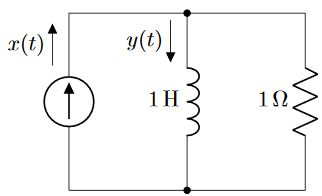
\includegraphics[scale=0.8]{RL.JPG}
        \caption{$RL$电路图}

    \end{figure}

\end{proposition}

\begin{proof}

    \begin{enumerate}

        \item 
            由图可知,$RL$电路的微分方程为
            \[\dfrac{\diff y(t)}{\diff t} + y(t) = x(t)\]
            当输入电流$x(t) = \euler^{-2t}u(t)$,且$y(0^{-}) = 0$时,微分方程的\textup{Laplace}变换为
            \[s\mathscr{Y}(s) + \mathscr{Y}(s) = \mathscr{X}(s) = \dfrac{1}{s + 2}\]
            \[\mathscr{Y}(s) = \dfrac{1}{(s + 1)(s + 2)} = \dfrac{1}{s + 1} - \dfrac{1}{s + 2}\]
            由变换对易知,电路的零状态响应为
            \[y(t) = \euler^{-t}u(t) - \euler^{-2t}u(t)\]

        \item 
            当输入电流$x(t) = 0$,且$y(0^{-}) = 0$时,微分方程的\textup{Laplace}变换为
            \[s\mathscr{Y}(s) - y(0^{-}) + \mathscr{Y}(s) = 0\]
            即
            \[\mathscr{Y}(s) = \dfrac{1}{s + 1}\]
            由\textup{Laplace}变换对易知,电路的零状态响应为
            \[y(t) = \euler^{-t}u(t)\]
        \item 
            当输入电流$x(t) =  \euler^{-2t}u(t)$,初始条件同\textup{(b)}时,
            微分方程的\textup{Laplace}变换为
            \[s\mathscr{Y}(s) - y(0^{-}) + \mathscr{Y}(s) = \mathscr{X}(s) = \dfrac{1}{s + 2}\]
            即
            \[\mathscr{Y}(s) = \dfrac{2}{s + 1}  - \dfrac{1}{s + 2}\]
            由\textup{Laplace}变换对易知,电路的零状态响应为
            \[y(t) = \euler^{-t}u(t) - 2\euler^{-2t}u(t)\]
    \end{enumerate}

    
\end{proof}


\begin{proposition}
    
    关于信号$x(t)$,已知以下三点:
    
    \begin{enumerate}

        \item $x(t) = 0$,$t < 0$
        
        \item $x \left( \dfrac{k}{80} \right) = 0$,$k = 1, 2, 3, \cdots$
        
        \item $x \left( \dfrac{1}{160} \right) = \euler^{-120}$
        
   \end{enumerate}

   设$X(s)$为$x(t)$的\textup{Laplace}变换,则$X(s)$在有限$s$平面内有几个极点。

\end{proposition}

\section{\texorpdfstring{$z$}{z}变换}

\begin{proposition}

    有一个信号$x[n]$的$z$变换的代数表达式为
    \[X(z) = \dfrac{1 + z^{-1}}{1 + \frac{1}{3}z^{-1}}\]

    \begin{enumerate}

        \item 假定收敛域是$|z| > \dfrac{1}{3}$,利用长除法求$x[0]$,$x[1]$和$x[2]$的值。
        
        \item 假定收敛域是$|z| < \dfrac{1}{3}$,利用长除法求$x[0]$,$x[1]$和$x[2]$的值。
        
    \end{enumerate}

\end{proposition}

\begin{proof}
    
    \begin{enumerate}

        \item \[(1 + z^{-1}) / \left( 1 + \frac{1}{3}z^{-1} \right) = \left( 1 + \dfrac{2}{3}z^{-1} - \dfrac{2}{9}z^{-2} \right)\]
        
        \item \[(z^{-1} + 1) / \left( \frac{1}{3}z^{-1} + 1 \right) = (3 - 6z^{1} + 18z^{2})\]

    \end{enumerate}

\end{proof}

